\section{Methods}
\label{sec:methods}

% NOT finished

\subsection{Dataset and SQI-based Data Selection}
\label{subsec:data_selection}
% almost finished

The public dataset for the Challenge is the International Cardiac Arrest REsearch consortium (I-CARE) database \cite{ICAREDatabase}. It contains mainly EEG recordings from comatose patients with cardiac arrest which were collected up to 72 hours from their return of spontaneous circulation (ROSC). Although this dataset contains physiological signals other than EEG, we base this study only on the EEG data for the following 2 reasons:
\begin{itemize}
    \item The amount of EEG data in the public dataset is already enormous, exceeding 30,000 hours in length.
    \item Previous literature \cite{Zheng_2021_coma} has illustrated the feasibility of using EEG as the sole physiological signal source on the problem this work considers.
\end{itemize}

As the computation resources and execution time are limited under the circumstances of the Challenge, further offline data selection was conducted according to the signal quality index (SQI) of the EEGs. The SQI was computed for every 5-minute epoch as its proportion of ``normal'' 10s segments. A 10s segment is regarded as ``normal'' if no artefact is detected from it, including abnormal values and patterns in the waveform and in the spectrum \footnote{Refer to \url{https://github.com/DeepPSP/cinc2023/utils/artifact_pipeline} for more details.}
% The distribution of SQI for all 5-minute epochs is collected in Figure \ref{fig:sqi-stats}.
At most one epoch was chosen (requiring SQI $\ge 0.95$) from each EEG recording as a representative of it for developing our neural network (NN) models (models will be discussed in Section \ref{subsec:models}). The total number of 5-minute epochs selected was 23350.

% \begin{figure}[!htp]
% \centering
% 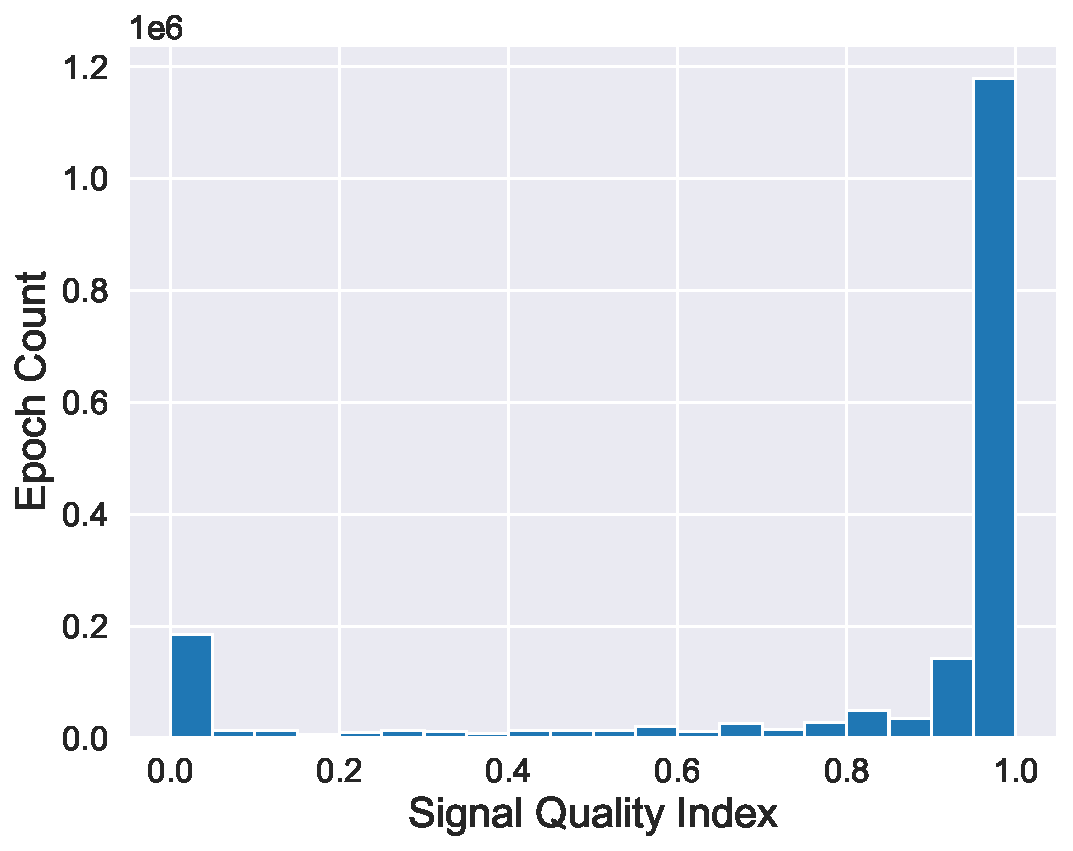
\includegraphics[width=0.95\linewidth]{images/sqi-stats.pdf}
% \caption[]{Distribution of SQI for all 5-minute EEG epochs. Consecutive epochs from one EEG recording have a 1-minute gap (hop length).}
% \label{fig:sqi-stats}
% \end{figure}


\subsection{Preprocessing Criteria}
\label{subsec:data_preproc}
% almost finished

In this subsection, we describe our preprocessing pipeline for model development and making inferences.

The EEG recordings provided by the I-CARE dataset have varying numbers (19 - 21) of channels but share a common set of 19 channels. The voltage values of each EEG signal are relative to an ``unknown'' reference potential. Hence in order to align these voltage values, the varying-dimensional EEG signals were transformed into the bipolar format with the following 18 channels
\begin{indentedquote}{0.3in}
\it Fp1-F7, F7-T3, T3-T5, T5-O1, Fp2-F8, F8-T4, T4-T6, T6-O2, Fp1-F3, F3-C3, C3-P3, P3-O1, Fp2-F4, F4-C4, C4-P4, P4-O2, Fz-Cz, Cz-Pz
\end{indentedquote}
Bipolar values were obtained by subtracting the latter channel from the former channel of the above 18 pairs.
% The number 18 was chosen since it's the smallest number of bipolar channels to reconstruct the original 19-channel EEG signal.

Bipolar EEGs were further standardized with the following 3 sequential operations:
\begin{itemize}
    \item resample to 100 Hz using polyphase filtering;
    \item Butterworth bandpass filter of order 4 and cutoff frequencies 0.5 - 30 Hz;
    \item rescale to zero mean and unit variance (also called z-score normalization).
\end{itemize}

It has to be emphasized that the z-score normalization is a crucial step, without which the model performance degraded significantly as observed in offline experiments which is demonstrated in Figure \ref{fig:train_scores_compare}.

\begin{figure}[!htp]
\centering
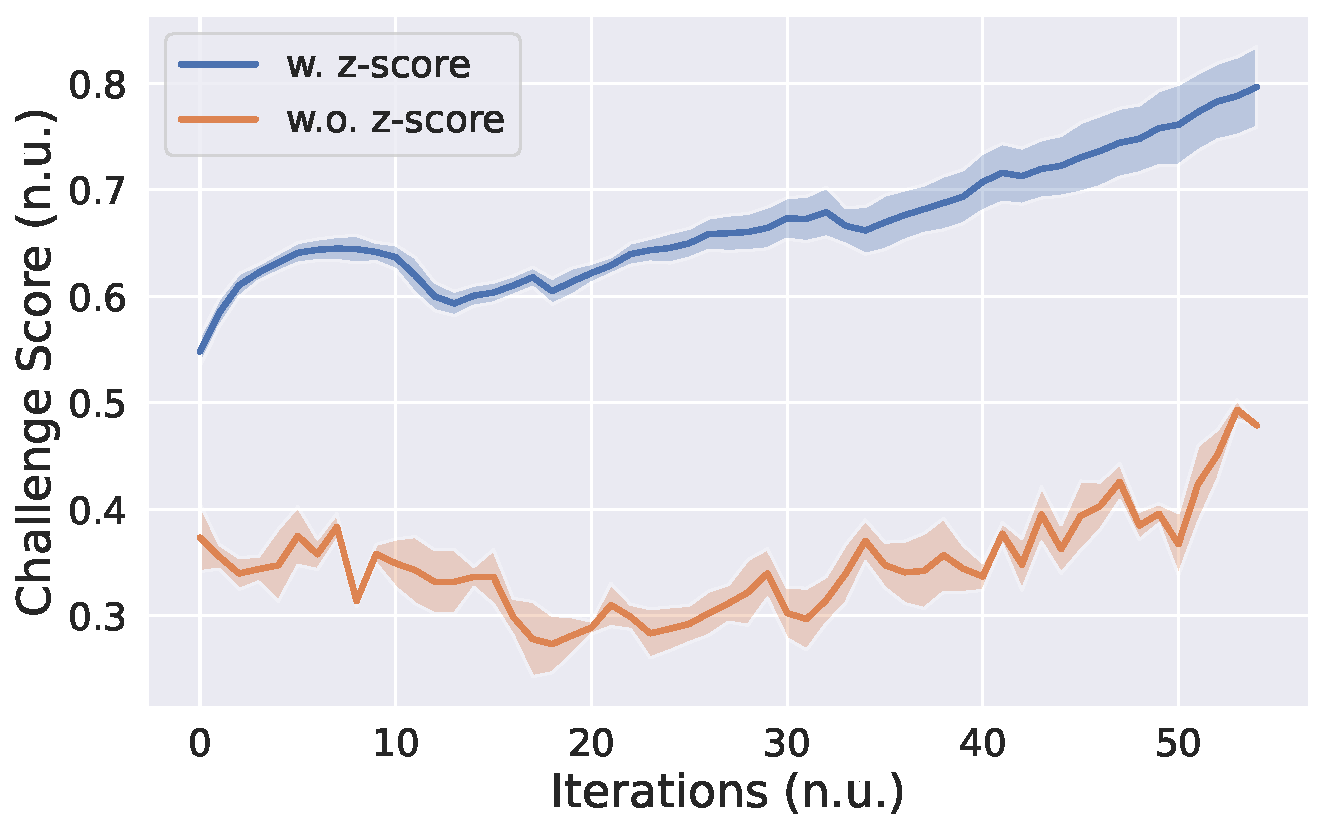
\includegraphics[width=0.95\linewidth]{images/train_scores_compare.pdf}
\caption[]{Comparison between mean curves of challenge scores from multiple experiments on the training set with (w.) and without (w.o.) z-score normalization. Shaded areas are error bounds (standard error of the mean).}
\label{fig:train_scores_compare}
\end{figure}

\subsection{Neural Network Model Selection}
\label{subsec:models}
% almost finished

Considering that there's a clear and widely accepted (also adopted in the Challenge) mapping from CPC scores to clinical outcomes as follows:
\begin{equation}
\label{eq:cpc_outcome_mapping}
\begin{array}{cl}
\text{``Good outcome''} & \text{for CPC score } \in \{1, 2\}; \\
\text{``Poor outcome''} & \text{for CPC score } \in \{3, 4, 5\},
\end{array}
\end{equation}
% \begin{itemize}
%     \item ``Good outcome'' for CPC score $\in \{1, 2\};$
%     \item ``Poor outcome'' for CPC score $\in \{3, 4, 5\},$
% \end{itemize}
and that the CPC scores are discrete scalars, we regard the problem as a 5-class classification problem, i.e. predicting the 5 discrete CPC scores.

A Time-incremental Convolutional Recurrent Neural Network (TiCRNN) \cite{Kang_2022_cinc2021_iop} was adopted as the CPC score classifier. Models with CRNN architecture, especially those with SE-ResNet \cite{hu2020senet} CNN backbones, have proven effective in various physiological signal processing tasks \cite{Kang_2022_cinc2021_iop, wen_cinc2022}. The building block of the SE-ResNet backbone used in this work consists of 3 sequential convolutional blocks of bottleneck shape followed by an SE (squeeze-and-excitation) block with an extra shortcut connecting the input and output as sketched in Figure \ref{fig:se_bottleneck}. The whole architecture of the TiCRNN model used in this work is depicted in Figure \ref{fig:model_arch}. It is a sequential model with 1 stem convolutional block which takes preprocessed EEG waveforms as input, 4 SE-Bottleneck blocks, 2 bidirectional LSTM blocks, 1 SE global attention module, 1 adaptive average pooling layer which outputs the feature vectors, and a multi-layer perceptron which takes in the feature vectors and outputs the probability vectors for the 5 CPC scores.

\begin{figure}[!htp]
\centering
\begin{figure}
\centering

\begin{tikzpicture}%[node distance = 1cm, auto]

\tikzstyle{block} = [rectangle, draw, text width = 5em, text centered, rounded corners, inner sep = 3pt, minimum height = 1.0em]

\tikzstyle{wideblock} = [rectangle, draw, text width = 12em, text centered, rounded corners, inner sep = 3pt, minimum height = 1.0em]

\tikzset{%
  do path picture/.style={%
    path picture={%
      \pgfpointdiff{\pgfpointanchor{path picture bounding box}{south west}}%
        {\pgfpointanchor{path picture bounding box}{north east}}%
      \pgfgetlastxy\x\y%
      \tikzset{x=\x/2,y=\y/2}%
      #1
    }
  },
  plus/.style={do path picture={    
    \draw [line cap=round] (-3/4,0) -- (3/4,0) (0,-3/4) -- (0,3/4);
  }}
}

\coordinate (top) at (0, 0);
\pgfmathsetmacro\blockdist {0.4}
\pgfmathsetmacro\pathshift {0.1}

\node [wideblock, below = \blockdist of top] (conv1) {Conv($n_1, m)$};
\path [->] (top) edge ([yshift = \pathshift]conv1.north);

\node [block, below = \blockdist of conv1] (conv2) {Conv($m, m)$};
\path [->] ([yshift = -\pathshift]conv1.south) edge ([yshift = \pathshift]conv2.north);

\node [wideblock, below = \blockdist of conv2] (conv3) {Conv($m, n_2)$};
\path [->] ([yshift = -\pathshift]conv2.south) edge ([yshift = \pathshift]conv3.north);

\node [wideblock, below = \blockdist of conv3] (se) {SE Block};
\path [->] ([yshift = -\pathshift]conv3.south) edge ([yshift = \pathshift]se.north);

\node [circle, draw, plus, below = 0.7 * \blockdist of se] (plus) {};
\path [->] ([yshift = -\pathshift]se.south) edge ([yshift = \pathshift]plus.north);

\coordinate[below = 0.7 * \blockdist of plus] (bottom);
\path [->] ([yshift = -\pathshift]plus.south) edge (bottom);

\node [block, above right = -0.2 and 0.6 of conv3] (shortcut) {Shortcut};
\draw [->] ([yshift = 7]conv1.north) -| ([yshift = \pathshift]shortcut.north);
\draw [->] ([yshift = -\pathshift]shortcut.south) |- ([xshift = \pathshift]plus.east);


\draw[rounded corners, dashed, thick] ([xshift = -70, yshift = -11]se) rectangle ([xshift = 70, yshift = 11]conv1);
\draw[rounded corners, ultra thick] ([xshift = -82, yshift = -5]bottom) rectangle ([xshift = 145, yshift = 5]top);

\end{tikzpicture}

\caption{The structure of an SE-Bottleneck block. The mainstream in the dashed box consists of 3 convolutional blocks (actually compositions of convolution, batch normalization and activation) followed by an SE block. The channels $n_1, n_2$ are typically several times of $m,$ hence giving the name ``bottleneck''. The shortcut is typically convolutions of kernel size 1, whose stride and input/output channels match the mainstream.}
\label{fig:se_bottleneck}
\end{figure}

\caption{The structure of an SE-Bottleneck block. The mainstream in the dashed box consists of 3 convolutional blocks (actually compositions of convolution, batch normalization and activation) followed by an SE block. The channels $n_1, n_2$ are typically several times of $m,$ hence giving the name ``bottleneck''. The shortcut is typically convolutions of kernel size 1, whose stride and input/output channels match the mainstream.}
\label{fig:se_bottleneck}
\end{figure}
\end{figure}

\begin{figure}[!htp]
\centering
% finished

\begin{tikzpicture}%[node distance = 1cm, auto]

% \tikzstyle{block} = [rectangle, draw, text width = 5em, text centered, rounded corners, inner sep = 3pt, minimum height = 1.0em]

\tikzstyle{wideblock} = [rectangle, draw, text width = 12em, text centered, rounded corners, inner sep = 3pt, minimum height = 1.0em]

\pgfmathsetmacro\blockdist {0.4}
\pgfmathsetmacro\pathshift {0.1}

\node [rectangle, text width = 12em, text centered, rounded corners, inner sep = 3pt, minimum height = 1.0em] (input) {EEG Waveform};

\node [wideblock, below = \blockdist of input] (stem) {Stem Conv};
\path[->] ([yshift = -\pathshift]input.south) edge ([yshift = \pathshift]stem.north);

\ifcoloredtext
\node [wideblock, below = \blockdist of stem] (bottleneck) {\bf\color{red}4 $\times$ SE-Bottleneck};
\path[->] ([yshift = -\pathshift]stem.south) edge ([yshift = \pathshift]bottleneck.north);
\else
\node [wideblock, below = \blockdist of stem] (bottleneck) {\bf 4 $\times$ SE-Bottleneck};
\path[->] ([yshift = -\pathshift]stem.south) edge ([yshift = \pathshift]bottleneck.north);
\fi

\node [wideblock, below = \blockdist of bottleneck] (lstm) {2 $\times$ Bidirectional LSTM};
\path[->] ([yshift = -\pathshift]bottleneck.south) edge ([yshift = \pathshift]lstm.north);

\node [wideblock, below = \blockdist of lstm] (se) {SE Global Attention};
\path[->] ([yshift = -\pathshift]lstm.south) edge ([yshift = \pathshift]se.north);

\node [wideblock, below = \blockdist of se] (pool) {Adaptive Average Pooling};
\path[->] ([yshift = -\pathshift]se.south) edge ([yshift = \pathshift]pool.north);

\node [wideblock, below = \blockdist of pool] (mlp) {Multi-Layer Perceptron};
\path[->] ([yshift = -\pathshift]pool.south) edge ([yshift = \pathshift]mlp.north);

\node [rectangle, text width = 12em, text centered, rounded corners, inner sep = 3pt, minimum height = 1.0em, below = \blockdist of mlp] (prob) {Probability Vectors for 5 CPC Scores};
\path[->] ([yshift = -\pathshift]mlp.south) edge ([yshift = \pathshift]prob.north);

\draw[rounded corners, dashed, thick] ([xshift = -80, yshift = -5]mlp.south) rectangle ([xshift = 80, yshift = 5]stem.north);
\ifboxednn
\draw[rounded corners, ultra thick] ([xshift = -103, yshift = -5]prob.south) rectangle ([xshift = 103, yshift = 5]input.north);
\fi

\end{tikzpicture}

\caption{Architecture of the TiCRNN model. Considering that the preprocessed input EEG waveforms have a sampling frequency of 100 Hz, convolutions, except the shortcuts in SE-Bottleneck blocks, have a kernel size of 3. The total number of trainable parameters in 92M.}
\label{fig:model_arch}
\end{figure}

Probability vectors from multiple EEGs of one patient are averaged and re-normalized via softmax to get the final CPC score predictions. The binary clinical outcomes (good, poor) are obtained by applying the mapping \eqref{eq:cpc_outcome_mapping}.

\subsection{Training Strategies}
\label{subsec:training}
% almost finished

As can be inferred from Figure \ref{fig:cpc_vfib_corr}, We have a highly imbalanced distribution of the learning objective (the CPC score) in the I-CARE dataset, which is also divergent across different hospitals as illustrated in Figure \ref{fig:outcome_hospital_corr}. Therefore, the asymmetric loss \cite{ridnik2021asymmetric_loss}, which is the state-of-the-art loss function for multi-label (and also for multi-class) classification problems, was chosen as the minimizing objective. The self-adaptive optimizer \texttt{AdamW} was used in conjunction with the \texttt{OneCycle} scheduler to incrementally update the NN model weights towards their optimal.

\begin{figure}[!htp]
\centering
\begin{subfigure}[t]{0.49\linewidth}
    \centering
    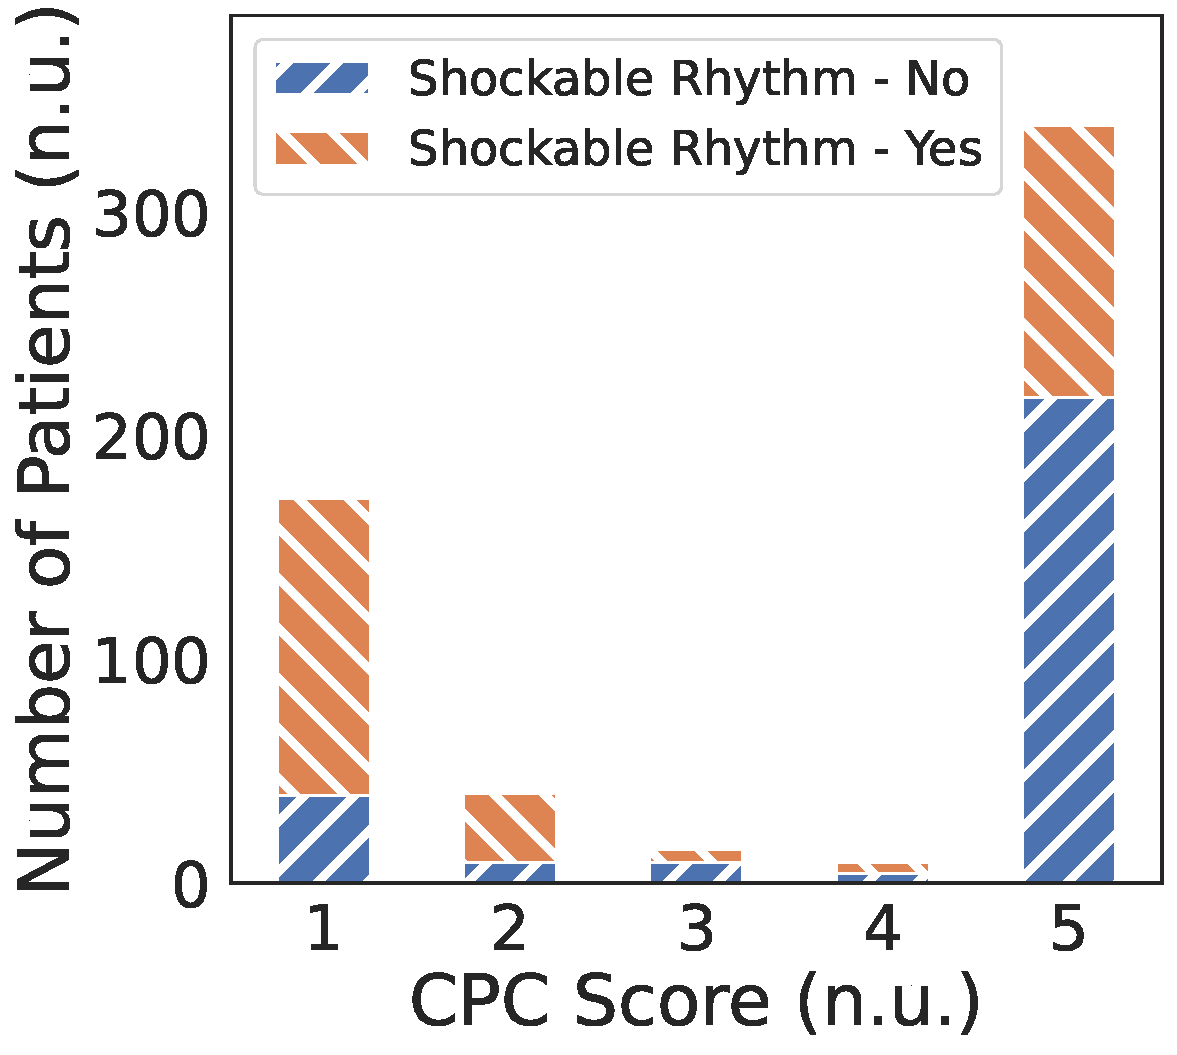
\includegraphics[width=\textwidth]{images/cpc-vfib-corr.pdf}
    \caption[]
    {Dist. against shockable rhythm.}
    \label{fig:cpc_vfib_corr}
\end{subfigure}
\hfill
\begin{subfigure}[t]{0.49\linewidth}
    \centering
    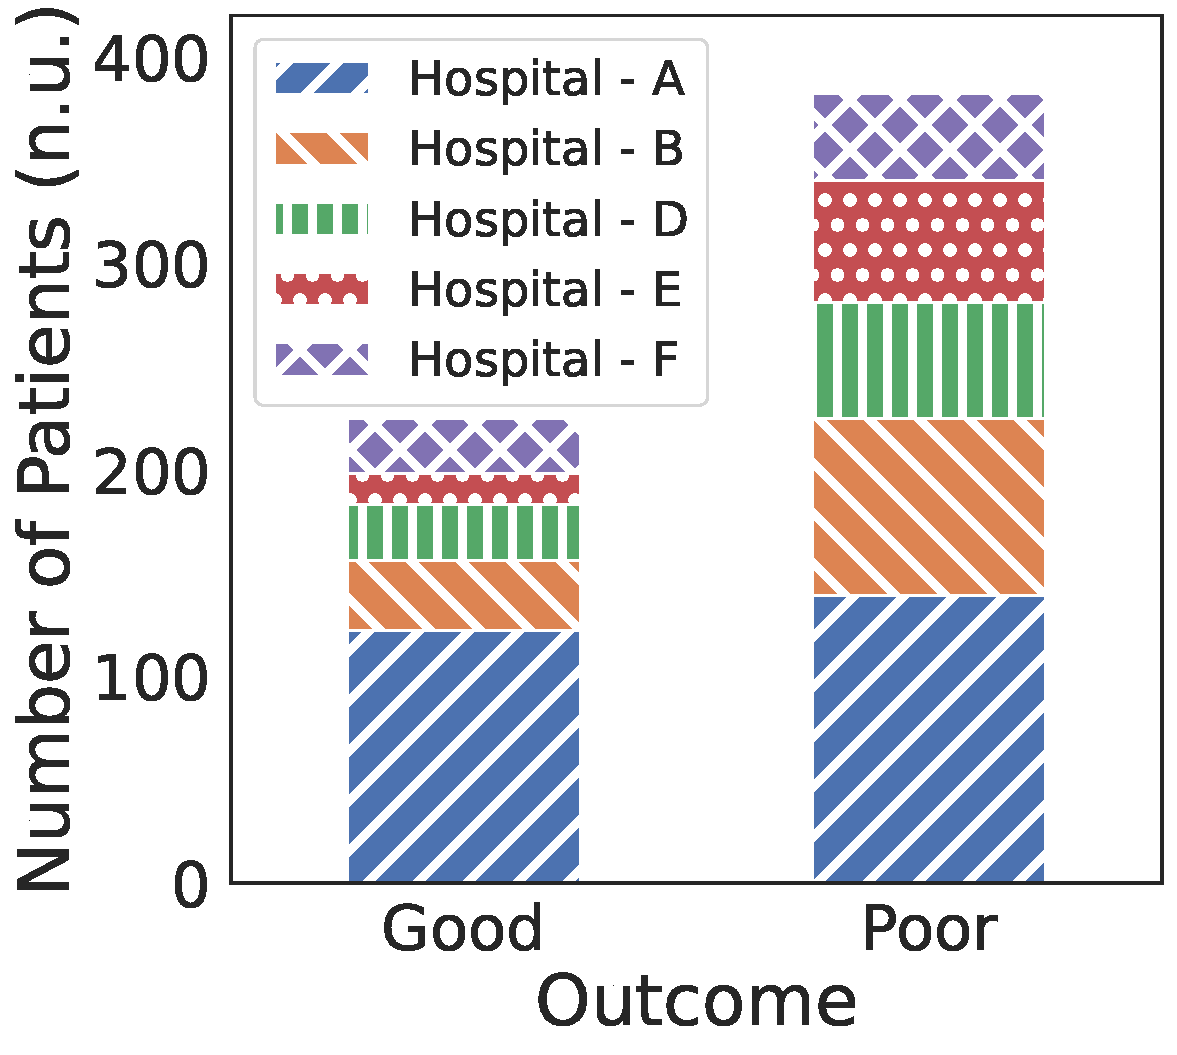
\includegraphics[width=\textwidth]{images/outcome-hospital-corr.pdf}
    \caption[]
    {Dist. against hospitals.}
    \label{fig:outcome_hospital_corr}
\end{subfigure}
\caption[]
{Distributions (Dist.) of the ``CPC Score'' and ``Outcome'' against 2 typical categorical metadata variables. Missing values for each variable were not counted.}
\label{fig:outcome_corr}
\end{figure}


The monitor for model selection is the Challenge score on a left-out validation set which was randomly selected and consisted of $20\%$ of the public training data. The Challenge score is defined as the largest TPR (true positive rate) such that FPR (false positive rate) $\le 0.05$ for the poor clinical outcome prediction. This agrees with the demand for methods with minimal false-positive rate of poor outcomes as introduced in Section \ref{sec:intro}.

A core contradiction for the Challenge lies in the conflict between the large data amount and the limited computation resources (RAM, execution time, etc.) as partly discussed in Section \ref{subsec:data_selection}. As a consequence, further trade-offs were made: we randomly sliced a 3-minute (180 in the number of sample points) piece from each of the selected 5-minute epochs and loaded all the data pieces into memory every 5 training iterations. The rest primary training hyperparameters are collected in Table \ref{tab:hyperparams}. It should be noted that the maximum number of training iterations was set to 55 since almost all optimal models were obtained before 30 iterations in our offline experiments using much larger total iteration numbers (e.g. 100 iterations).

\begin{table}[!htp]
\centering
% requires packages boldline, multirow
\setlength\tabcolsep{2pt}
\begin{tabular}{@{\extracolsep{6pt}}c|c|c|c|c@{}}
\hlineB{3.5}
\multirow{2}{*}{batch size} & max & early stop & \multicolumn{2}{c}{learning rate} \\ \cline{4-5}
& \# iterations & patience & initial & max \\ \hline
32 & 55 & 25 & 2.5e-3 & 8e-3 \\
\hlineB{3.5}
\end{tabular}
\caption{Primary hyperparameters for NN model training. To avoid overfitting on the training data, early stop callbacks were set which were triggered if the best Challenge score on the left-out validation set stayed unchanged for 25 global iterations. The learning rates were set for the optimizer and its scheduler.}
\label{tab:hyperparams}
\end{table}



% \subsection{Minimum Guarantee Models}
% \label{subsec:min_grt_models}
% % almost finished

% The Challenge also evaluated the submissions on subsets with recordings truncated up to 12 / 24 / 48 hours from ROSC, in which case a single patient might not have valid EEGs. In order to be able to predict clinical outcomes without EEGs, we used a random forest model as a minimum guarantee model which took all clinical information of a patient provided by the I-CARE database as input. This model was selected via parameter grid searching over the same train-validation split as described in Section \ref{subsec:training}.
